\documentclass[10pt,a4paper]{article}
\usepackage[latin1]{inputenc}
\usepackage{amsmath}
\usepackage{amsfonts}
\usepackage{amssymb}
\usepackage{color}
\usepackage{graphicx}
\usepackage{hyperref}
\usepackage{enumitem}
\usepackage{graphicx}
\hypersetup{
	colorlinks=true,
	linkcolor=blue,
	filecolor=magenta,
	urlcolor=cyan,
}
\RequirePackage[left=01.1cm,top=3cm,right=1.5cm,bottom=2.5cm,nohead,nofoot]{geometry}

\author{Anirudh ,Somesh ,Raina Thomas}

\title{
	\textbf{Scientific Experimentation and Evaluation}
	}
	
			
\begin{document}
	
\begin{titlepage}

	\maketitle
	
\end{titlepage}
\Large
\begin{enumerate}[label=\Roman*]
\item
\vspace{0.5cm}
\Large{\textbf{Aim}}\\

To construct a LEGO NXT differential drive robot and manually measure the observable  end pose variation for three different trajectories: an arc to the left, driving straight and an arc to the right.
\vspace{0.5cm}
\item
\Large{\textbf{Procedure}}\\

\begin{enumerate}
	\item
	The lego robot, which is the device under test(DUT), is built with a pen mounted in the front, back or the center of the robot.
	\item
	The measurement system is made of the robot, scale and a paper. The scale is used to measure the end pose of the robot relative to the start pose. The path taken by the robot is sketched on the paper by the pen.
	\item
	The initial pose of the robot is manually marked at the beginning along with the alignment of the wheels to measure the angular displacement at the final pose.
	\item
	The robot is programmed to move using the initial pose and the desired final pose.
	\item
	The measurands are the distance between the initial and end positions and the angles between the two poses.
	\item
	20 measurements would be performed for each trajectory. Mean and standard deviation will be computed from the measurement. These measured values would be used to compute the accuracy and precision of the pose variation. 
\end{enumerate}
\vspace{0.5cm}
\item
\textbf{Expected Problems}\\
\begin{enumerate}
	\item
	There could be slip in wheels.
	\item
	The pen could wobble and affect the shape of the curve and thereby the result.
	\item
	There will be errors in gears of the actuators such as backlash.
	\item
	Uneven surface of the paper could cause change in trajectory.
\end{enumerate}
\newpage	
\item
\textbf{Expected Performance}\\
\begin{enumerate}
	\item
	The slipping of wheels and the uneven surface of the paper could result in inaccurate results.
	\item
	The precision would not be perfect, but could have a small range since the DUT and the measurement facility are not changed.
	\item
	The accuracy depends strongly on the problems listed in section III. The most important problems would be the error due to wheel slip. Since the distance driven is maximum 1m, the error in precision and accuracy will lie in the centimeter range.
\end{enumerate}
\item
\textbf{Reference Images}\\

The reference images of the DUT and the proposed marker tracking visualization are given below.

\begin{figure}[h]
	\centering
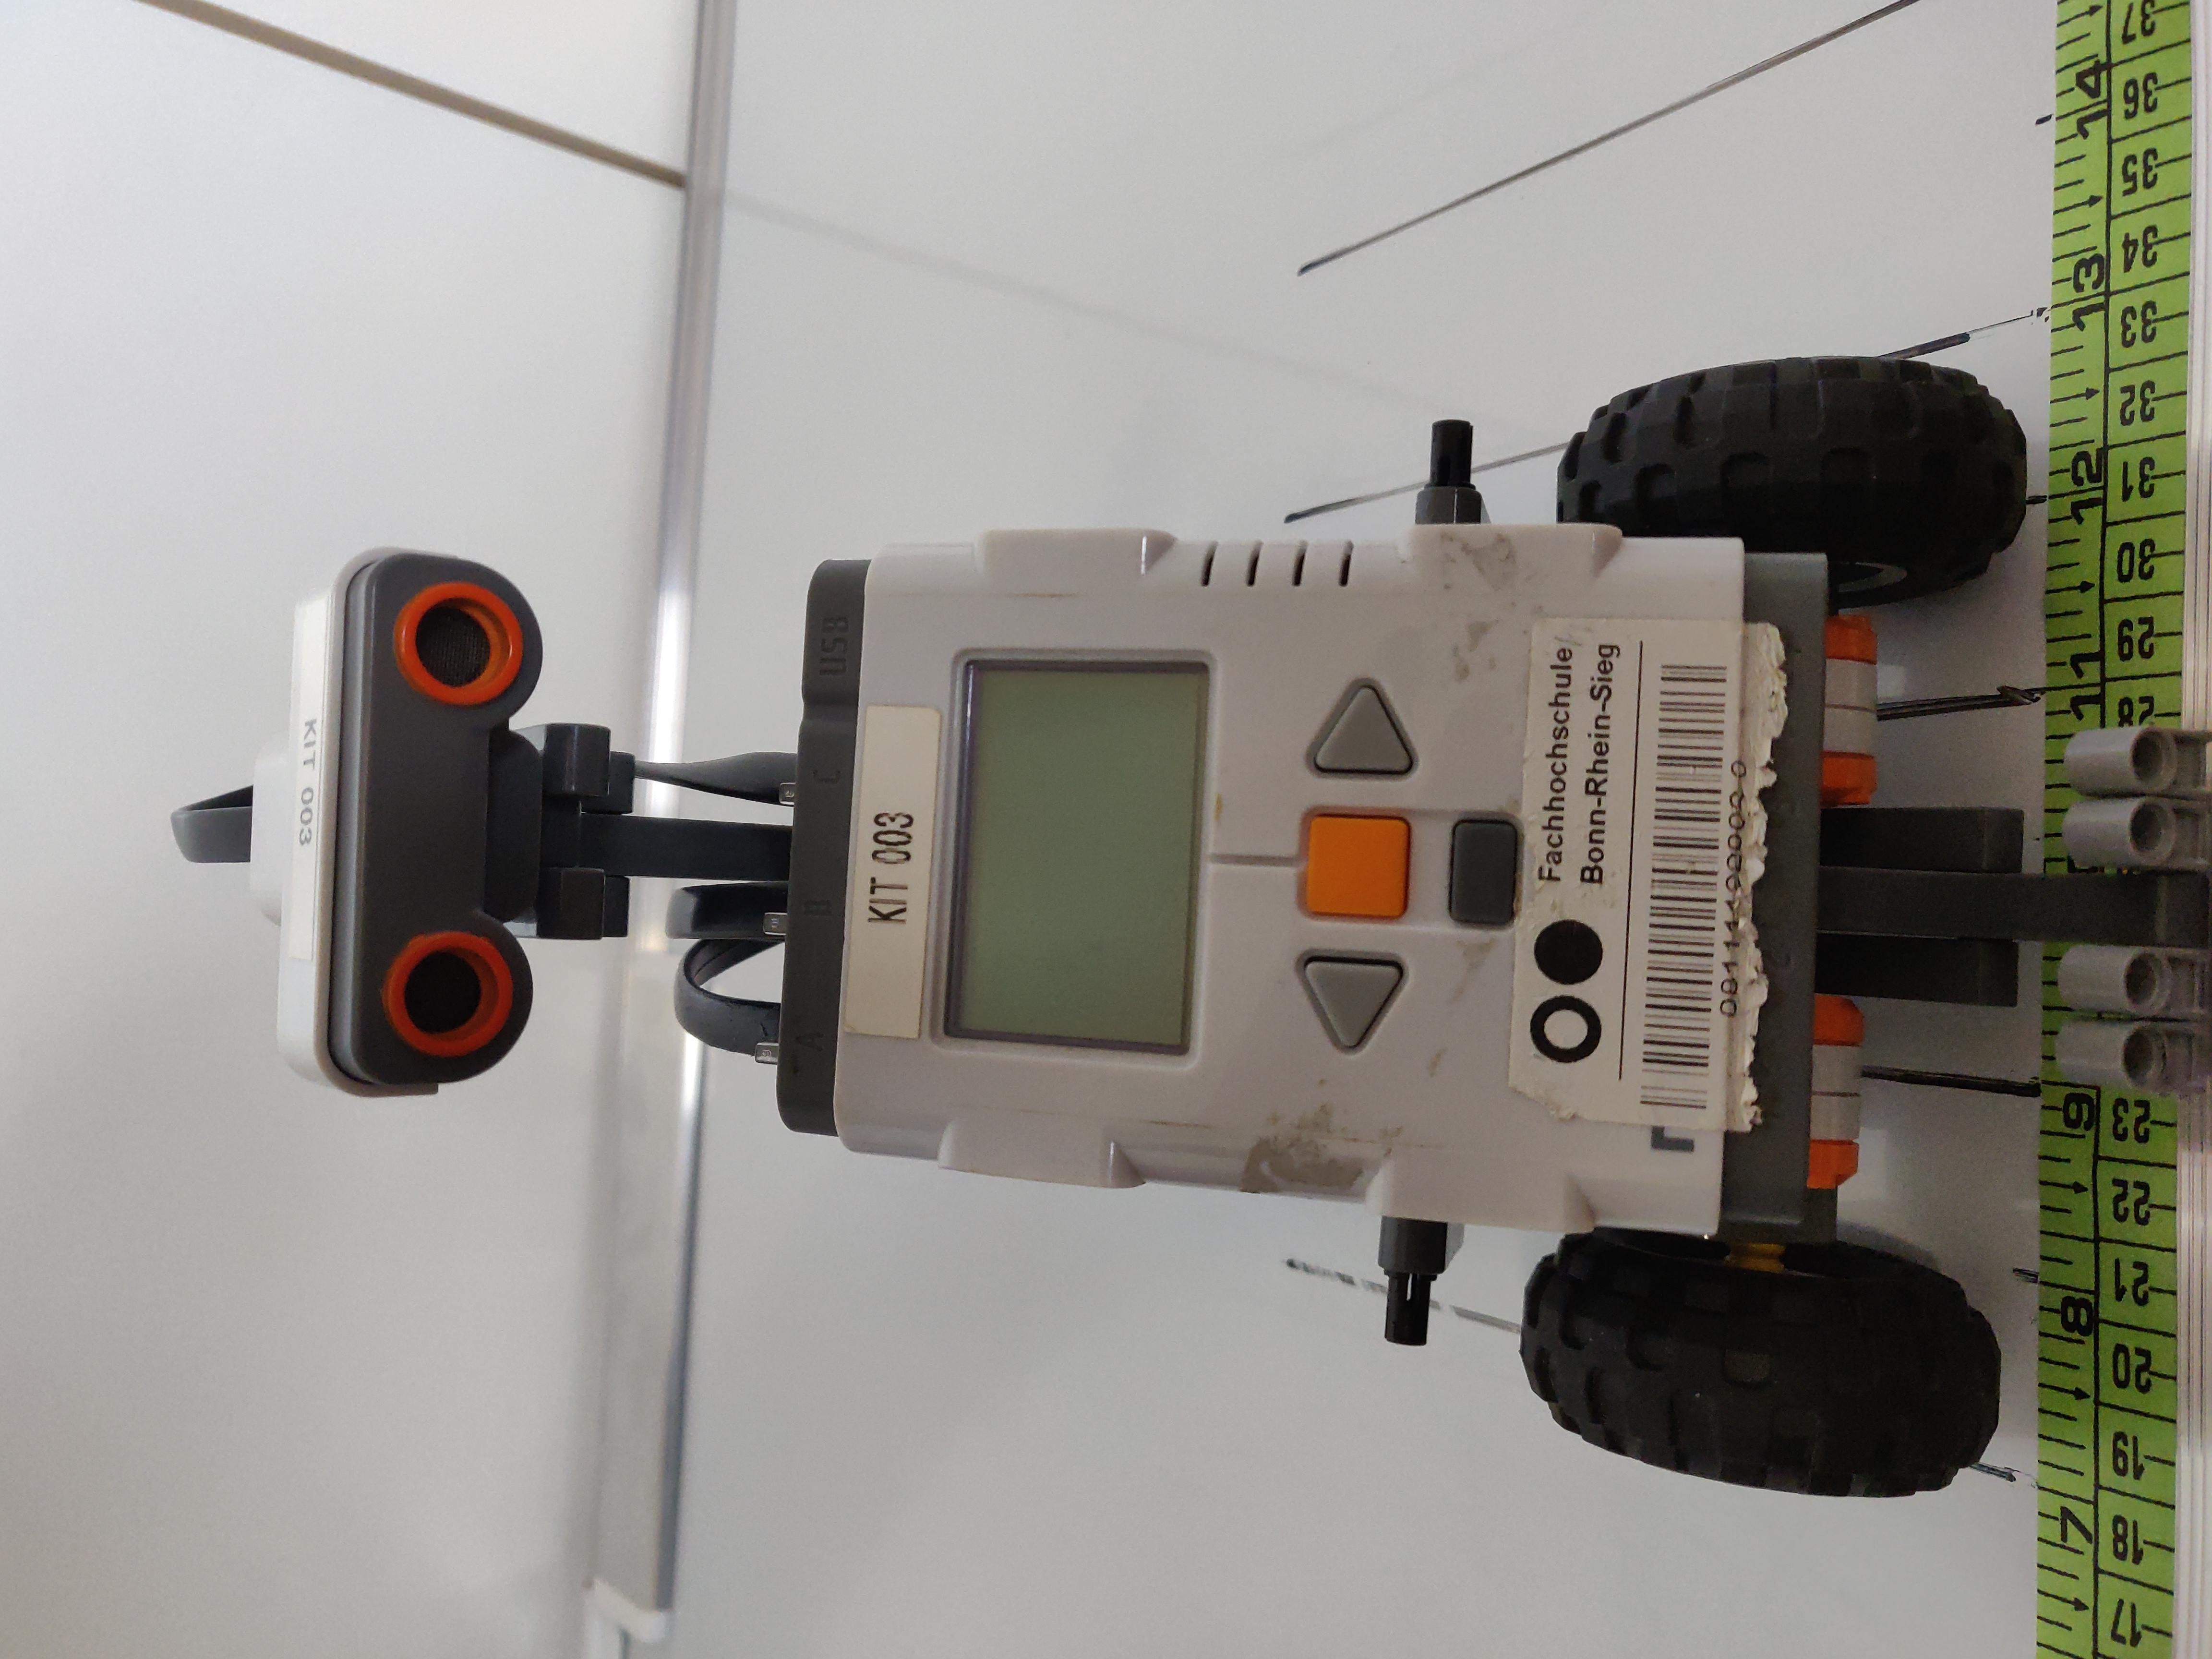
\includegraphics[width=0.7\linewidth, angle = -90 ]{Front_view}
\caption{ Front View of the DUT}
\end{figure}

\begin{figure}[h]
	\centering
	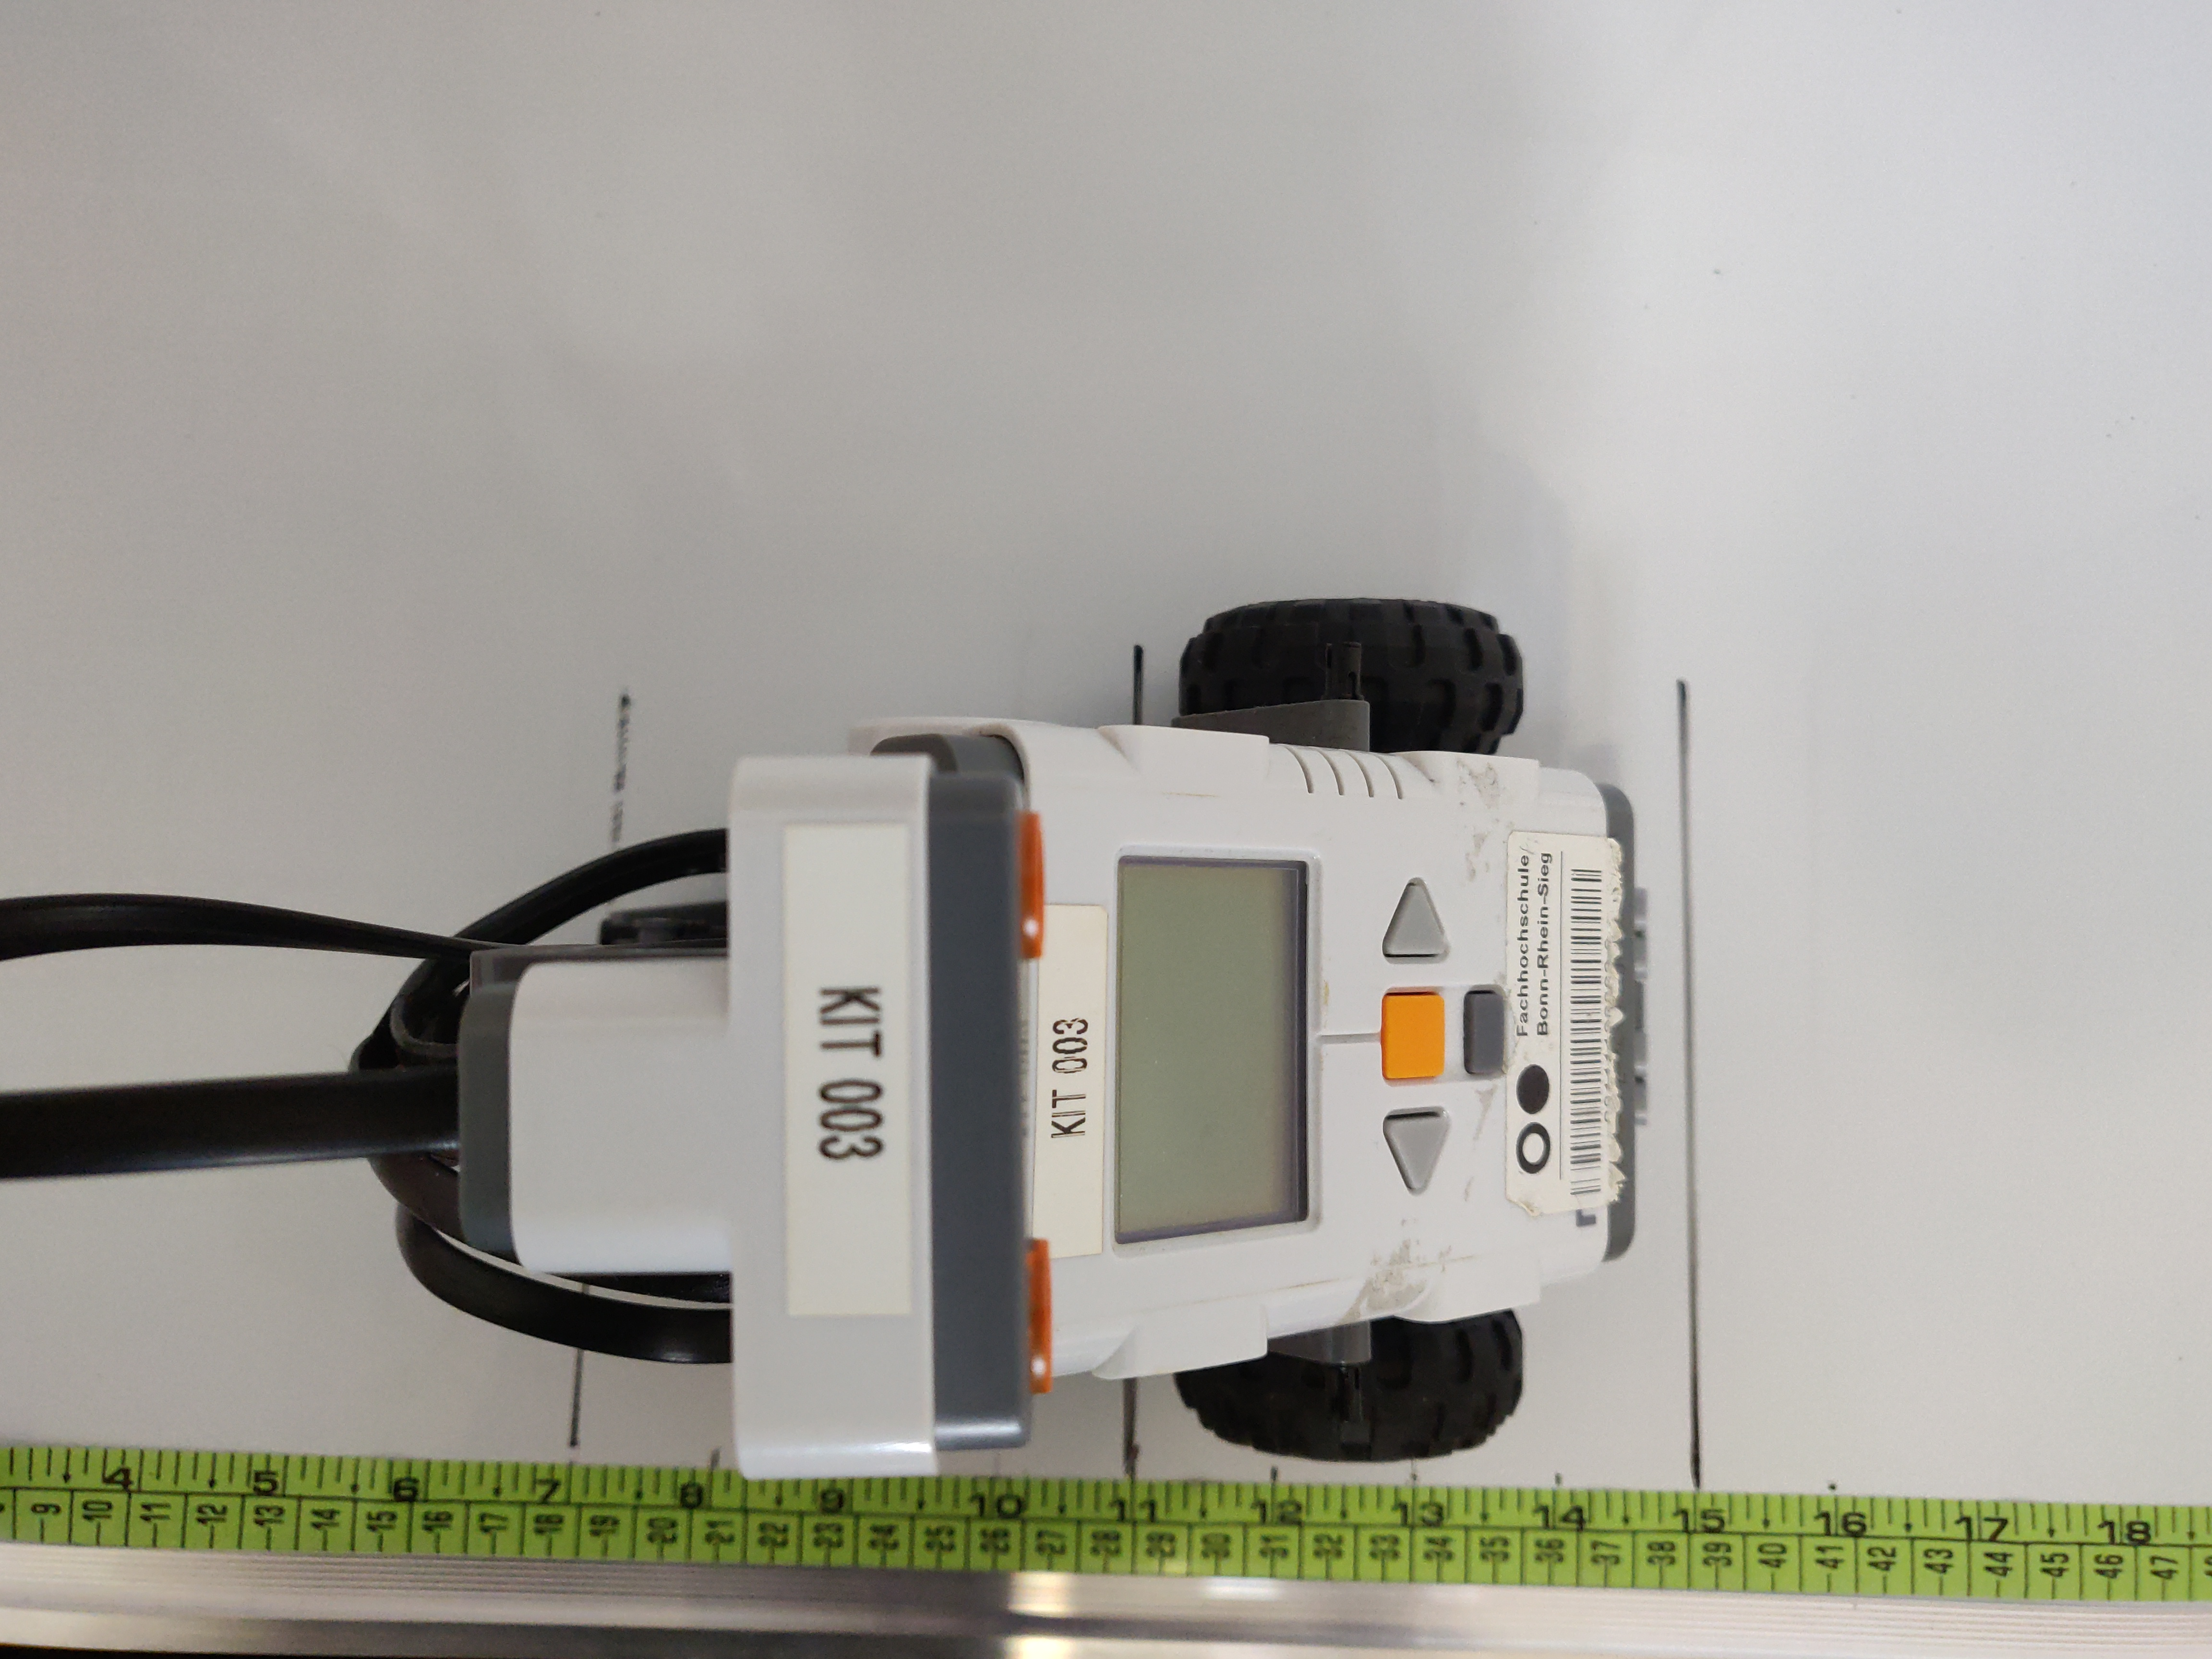
\includegraphics[width=0.7\linewidth, angle = -90]{Top_view}
	\caption{ Top View of the DUT}
\end{figure}

\begin{figure}[h]
	\centering
	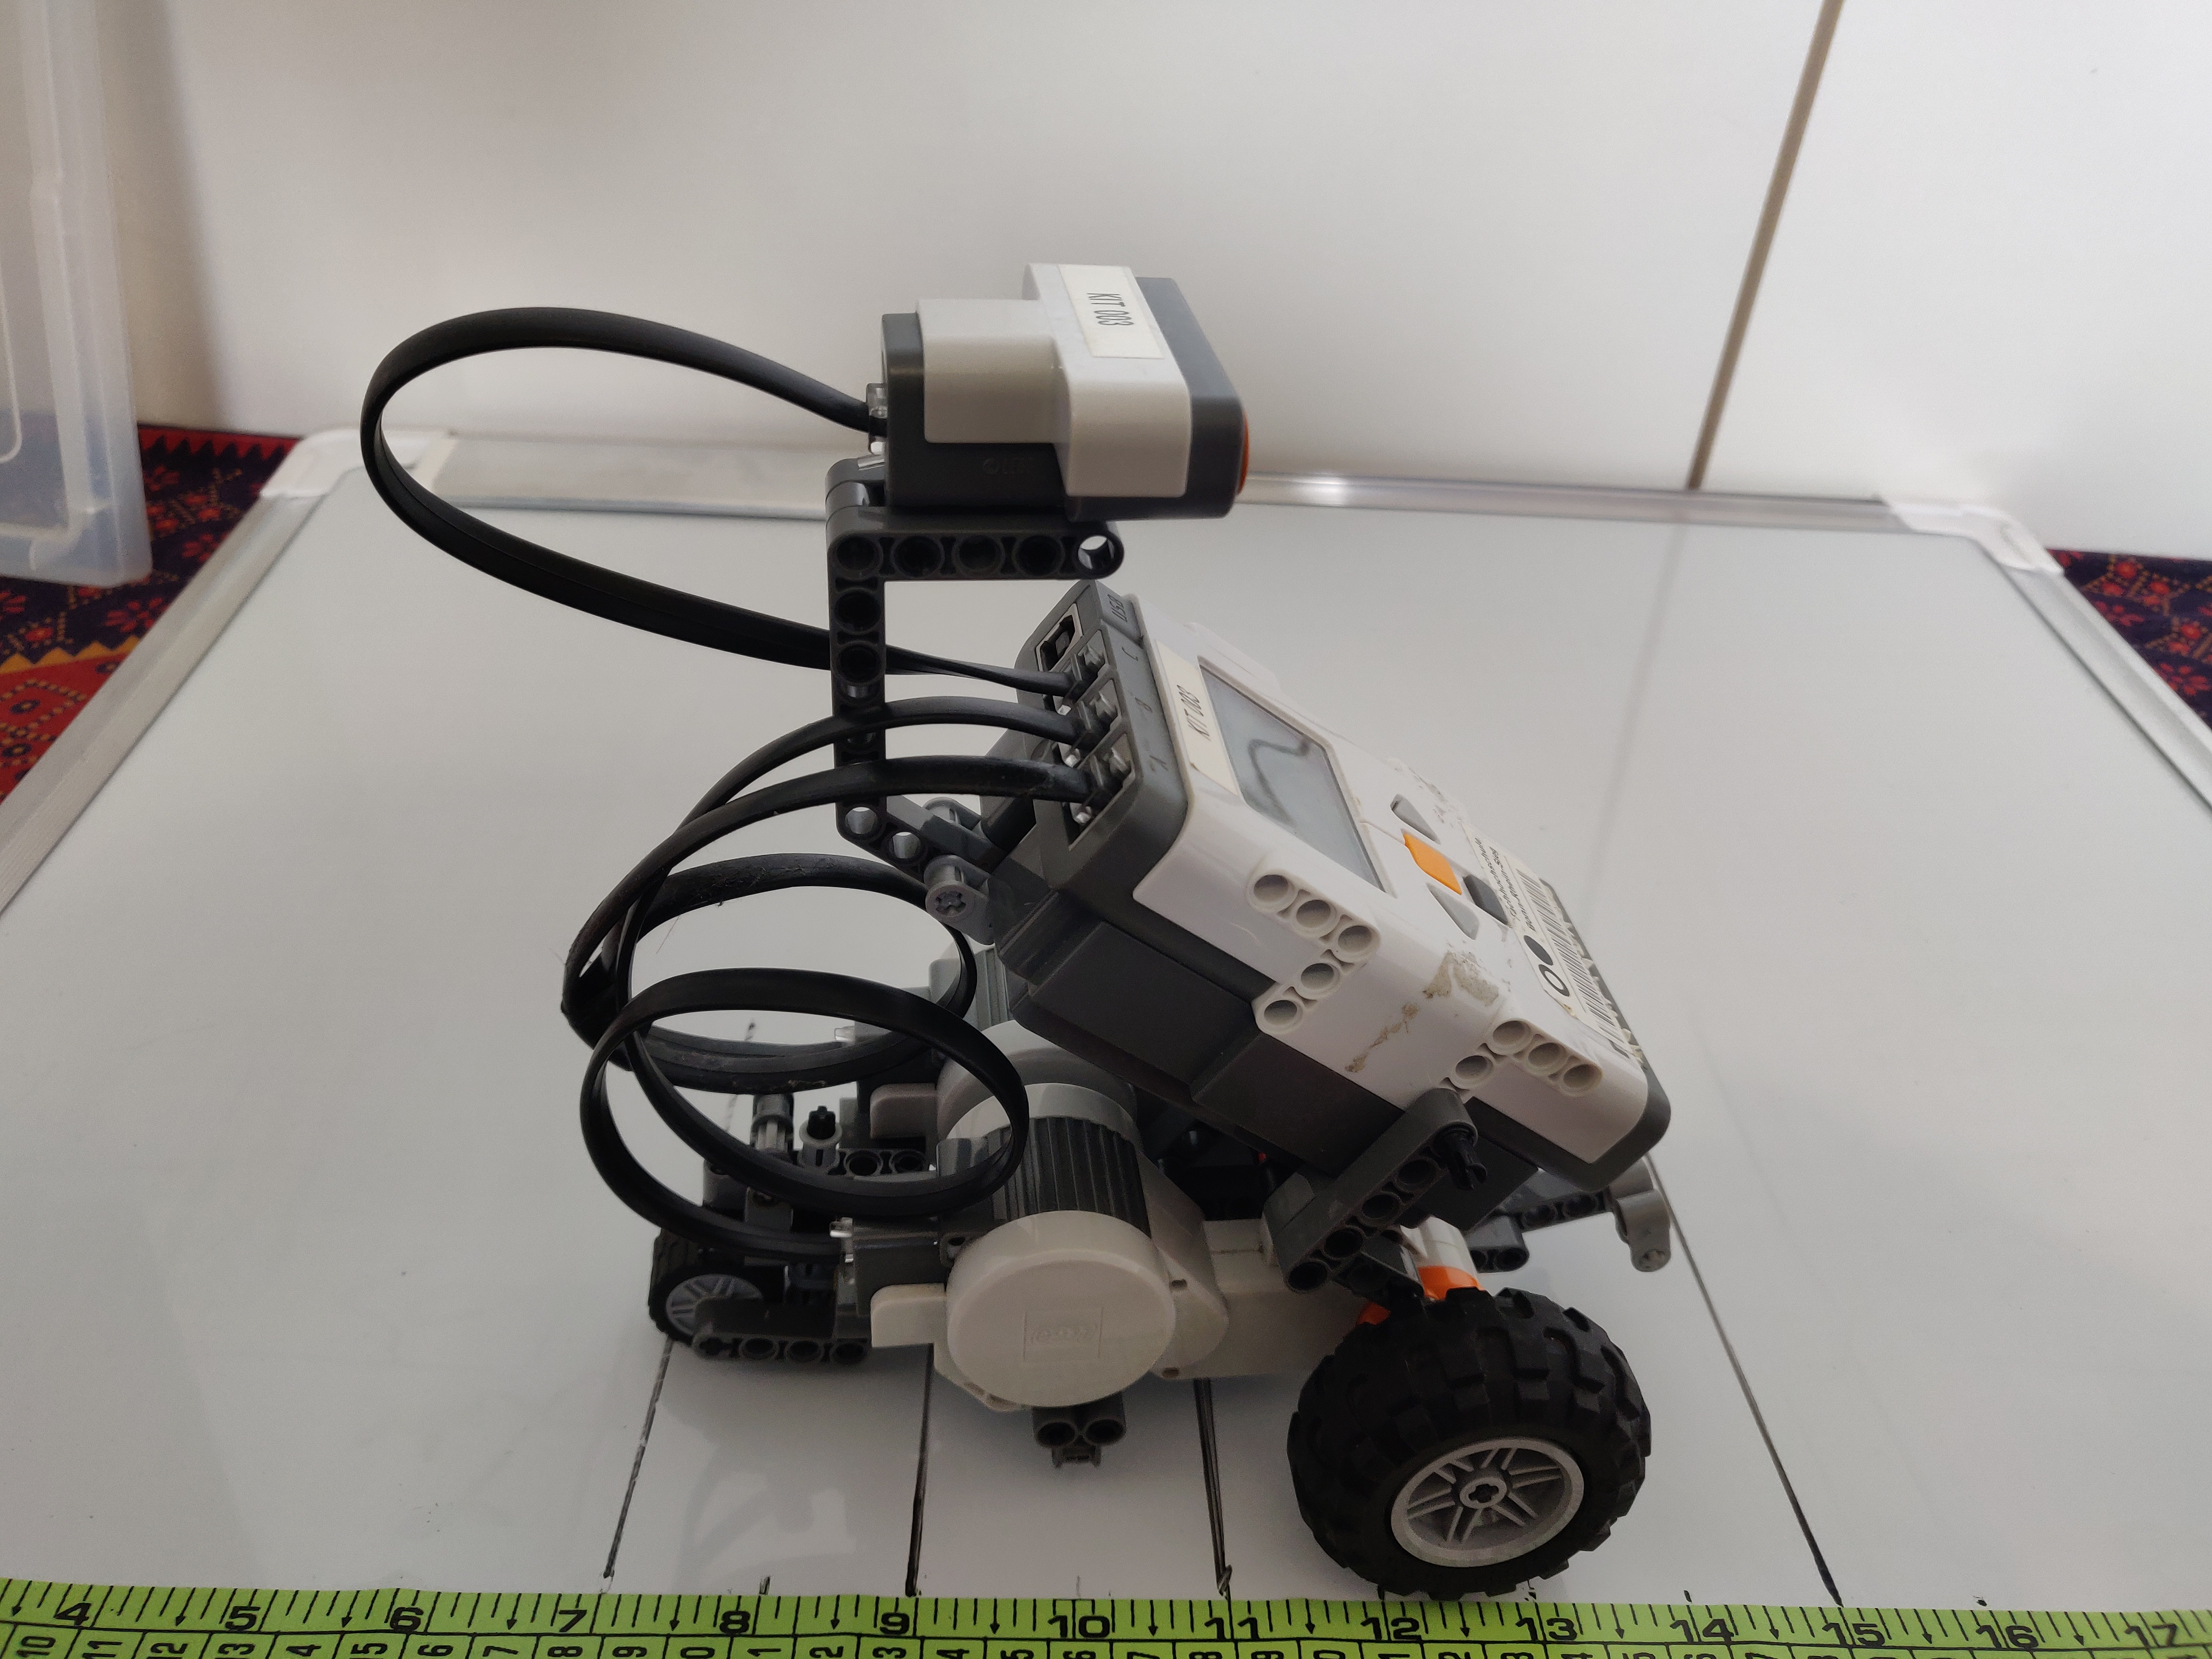
\includegraphics[width=0.7\linewidth]{Side_view}
	\caption{ Side View of the DUT}
\end{figure}
	

\end{enumerate}	






\end{document}


